\documentclass[11pt, a4paper]{article}

\usepackage{amsmath}
\usepackage{amsfonts}
\usepackage{graphicx}
\usepackage[export]{adjustbox}
\usepackage{hyperref}
\usepackage{fullpage}
\usepackage{caption}
\usepackage{listings}
\usepackage[dvipsnames]{xcolor}
\usepackage{gensymb}
\usepackage{wrapfig}
\hypersetup{
    bookmarks=true,         % show bookmarks bar?
    unicode=false,          % non-Latin characters in Acrobat’s bookmarks
    pdftoolbar=true,        % show Acrobat’s toolbar?
    pdfmenubar=true,        % show Acrobat’s menu?
    pdffitwindow=false,     % window fit to page when opened
    pdfstartview={FitH},    % fits the width of the page to the window
    pdftitle={My title},    % title
    pdfauthor={Author},     % author
    pdfsubject={Subject},   % subject of the document
    pdfcreator={Creator},   % creator of the document
    pdfproducer={Producer}, % producer of the document
    pdfkeywords={keyword1, key2, key3}, % list of keywords
    pdfnewwindow=true,      % links in new PDF window
    colorlinks=true,       % false: boxed links; true: colored links
    linkcolor=Blue,          % color of internal links (change box color with linkbordercolor)
    citecolor=green,        % color of links to bibliography
    filecolor=magenta,      % color of file links
    urlcolor=red           % color of external links
}

\title{MAAS - Street Network Visualization \\Group: Commitment\_Issues}
\author{Sushant Vijay Chavan\\Ahmed Faisal Abdelrahman\\Abanoub Abdelmalak}
\date{\today}

\begin{document}
\maketitle
\newpage
\tableofcontents{}
\newpage

\section{Introduction}
\paragraph{}
This document contains a brief overview of the street network graph visualization agent developed by this group. The agent facilitates displaying the street network map and the activity of truck agent in it in a JavaFX GUI. The agent was developed collectively by all team members, and its development involved several stages of additions and adjustments to the code.

%\newpage
\section{The Graph Visualization Agent}\label{GraphVisualizationAgent}
\paragraph{}
The graph visualization agent facilitates observing the delivery process of the orders in a graphical way. This agent is capable of displaying the entire street network (consisting of its nodes and edges) and all the trucks present at any given time as shown in figure \ref{VisualizationScreenshot}. JavaFX was used to generate the nice display and we used and modified the implementation of \href{https://stackoverflow.com/a/30696075}{Roland} to generate the graph representation.

\begin{figure}[h!]
	\centering
	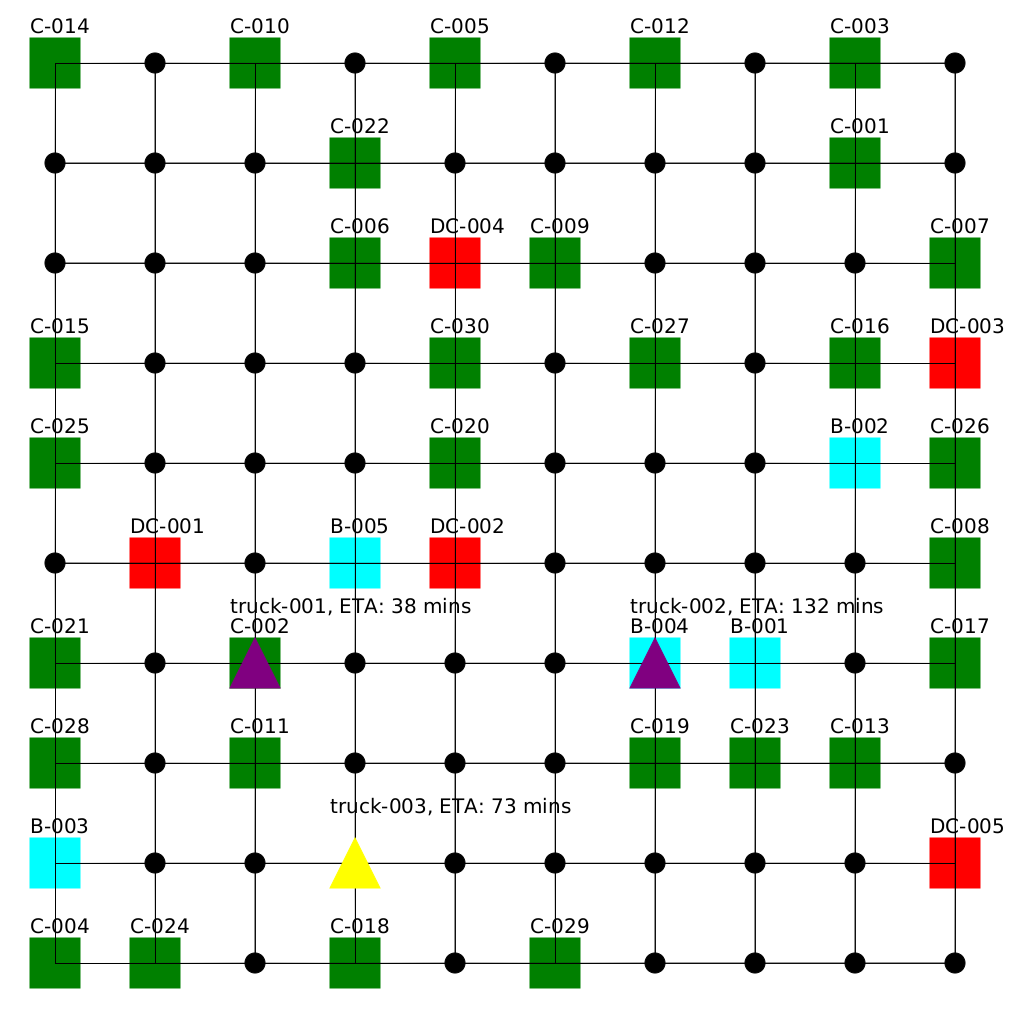
\includegraphics[width=\textwidth]{Visualization.png}
	\caption{Screenshot of Delivery Stage Visualization}
	\label{VisualizationScreenshot}
\end{figure}

\paragraph{}
The nodes of the graph are displayed as either squares (for important nodes such as bakery or customer locations) or small circles. The nodes are then connected by the edges. The squares are further color coded in order to distinguish the type of node. Green represents customers, red delivery companies and cyan bakery locations. The trucks are represented using triangles on the graph and it is possible to update their location based on their actual position in the graph at any time step. Similar to the nodes, the trucks are also color coded to identify their states. Gray represents idle state, yellow moving towards bakery for collecting boxes and purple delivering boxes to a customer. Additionally, the trucks also display the expected time of arrival along their current route.

\paragraph{}
This agent communicates with two agents in the delivery stage. The street network agent sends the street network information (consisting of the nodes and the edges) at startup to the graph visualization agent. Similarly, the trucks inform the graph visualization agent about their start positions. Whenever the position of a truck is updated, a new message is sent to the graph visualization agent informing it about the new position, expected time of arrival and state of the truck.


\section{Incoming Message Specifications}\label{MessageSpecifications}
\paragraph{}
The graph visualization agent uses the following message formats to communicate with the other two agents.

\hfill\break
\textbf{Message Descriptions}:

\hfill\break
\textbf{(Incoming) Street Network Message:}

\hfill\break
\textbf{Description}:
The Graph Visualization Agent receives the street network information from the Street Network Agent in a message of the following format:
\hfill\break
\textbf{Performative}: INFORM
\hfill\break
\textbf{Sender}: AID of the StreetNetworkAgent
\hfill\break
\textbf{Receiver}:  AID of the GraphVisualizationAgent
\hfill\break
\textbf{Conversation ID}: "graph-visualization"

\hfill\break
Figure \ref{graphVisSNmsgexample} shows an example of the contents of the message.

\begin{figure}[h!]
	\centering
	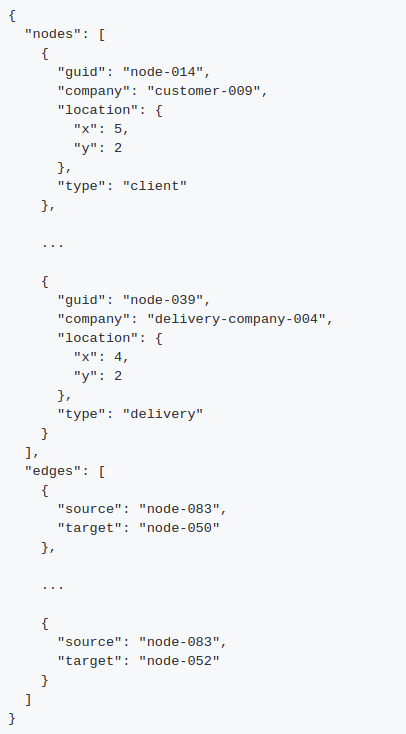
\includegraphics[width=0.5\textwidth]{../images/graphVisSNmsgexample.png}
	\caption{Incoming Street Network Message Example}
	\label{graphVisSNmsgexample}
\end{figure}


\hfill\break	
\textbf{(Incoming) Truck Message:}

\hfill\break
\textbf{Description}:
The Graph Visualization Agent receives the truck status information from the Truck Agent in a message of the following format:
\hfill\break
\textbf{Performative}: INFORM
\hfill\break
\textbf{Sender}: AID of the TruckAgent
\hfill\break
\textbf{Receiver}: AID of the GraphVisualizationAgent
\hfill\break
\textbf{Conversation ID}: "TruckPosUpdate"

\hfill\break
Figure \ref{graphVisTruckmsgexample} shows an example of the contents of the message.

\begin{figure}[h!]
	\centering
	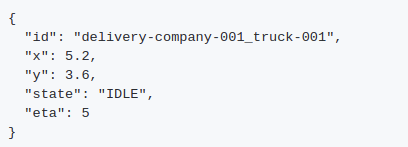
\includegraphics[width=0.5\textwidth]{../images/graphVisTruckmsgexample.png}
	\caption{Incoming Truck Message Example}
	\label{graphVisTruckmsgexample}
\end{figure}

\pagebreak
\newpage

\section{Running the Visualization}
\paragraph{}
The visualization of the delivery phase can be run by simply providing the `\textit{-visualization}' argument to the common \textit{gradle run} command. This automatically sets up the graph visualization agent which then communicates with the street network and the truck agents. In addition, the GUI window appears.

\paragraph{}
The same commands described in the team's report must be followed:
\begin{enumerate} 
	\item Start the program using the command
	\begin{verbatim}
	gradle run --args='-packaging -delivery -visualization'
	\end{verbatim}
	\item If you get an error saying gradle does not support '\textit{args}'. Then use the below command instead to start the program
	\begin{verbatim}
	./gradlew run --args='-packaging -delivery -visualization'
	\end{verbatim}
\end{enumerate}

\end{document}\grid
